\section{课程设计概述}
\subsection{设计目标与任务要求}

本课程设计主要分为云计算平台搭建和并行编程实战两部分。项目在华为云环境中完成应用容器化、镜像推送、Kubernetes 集群部署、Spark 数据分析和性能对比等工作。与只在本地运行脚本不同，本项目需要把容器、Service、LoadBalancer、PVC、ConfigMap、HPA 和 Spark 作业放到真实 CCE 环境中验证，因此报告重点记录配置过程、截图证据和排错依据。

任务书将课程设计划分为“云计算平台搭建”和“并行编程实战”两项主体任务，并将报告质量作为独立评分内容。其中，第一部分满分 50 分，要求在华为云 CCE 上部署“Flask 后端 API + Redis 数据库”两层 Web 应用，并完成应用容器化、CCE 集群搭建、Kubernetes 应用部署、Redis 持久化存储、ConfigMap Volume 挂载以及 HPA 弹性伸缩验证。第二部分满分 40 分，要求在第一部分建立的 Kubernetes 平台上选择 Spark 大数据分析或 MPI 并行科学计算方向完成并行编程实践。本项目选择方向 A，即 Spark 大数据分析，并围绕数据清洗、Spark SQL 统计分析、性能对比和 Amdahl 定律分析展开。报告质量部分满分 10 分，重点考查结构完整性、截图清晰度、图表规范性和结果分析深度。

\subsubsection{总体设计目标}

本项目的目标是让 Web 应用和 Spark 分析任务都能在云端正常运行，并留下可以复验的截图和配置文件。在平台层面，后端服务、Redis 和前端静态页面分别构建为容器镜像，再通过 Kubernetes Deployment、Service、ConfigMap、Secret、PVC 和 HPA 完成部署。在数据计算层面，项目选择 Spark 大数据分析方向，利用 PySpark 对电影数据进行清洗、聚合统计、趋势分析和性能测试。

图 \ref{fig:overall-architecture} 给出了本项目的总体架构。在线应用链路以 ELB 和 \verb|backend-svc| 为公网请求入口，请求由 Service 转发至两个 Flask 后端副本，后端再通过集群内部的 \verb|redis-svc| 访问 Redis；Redis 数据目录由 PVC 提供持久化存储。Nginx 前端通过反向代理复用后端 Service，ConfigMap、Secret 与 HPA 分别承担配置注入、敏感信息管理和副本弹性调节。离线分析链路则由 Spark Operator 在同一 CCE 集群中调度 Driver 与 Executor，读取 OBS 或实验数据集并输出统计与性能分析结果。两条链路共享 Kubernetes 计算环境，但在服务入口、状态存储和任务调度方面保持职责分离。

\reportfig[\textwidth]{figures/course-architecture.png}{课程设计总体架构与关键数据流}{fig:overall-architecture}

从能力培养角度看，本课程设计旨在形成以下几方面的综合实践能力：第一，能够根据任务书模板修改 Dockerfile 和应用配置，完成本地构建、联调与镜像推送；第二，能够在华为云 CCE 中创建满足版本和节点数量要求的 Kubernetes 集群，并使用 kubectl 进行资源管理与状态核验；第三，能够合理使用 ConfigMap、Secret、PVC、LoadBalancer 和 HPA 等资源解决配置分离、敏感信息管理、数据可靠性、外部访问和弹性伸缩问题；第四，能够在 Kubernetes 环境中运行 Spark 作业，并使用 Spark DataFrame 与 SQL API 完成数据分析任务；第五，能够基于截图、日志、实验数据和理论模型对实验结果进行解释，而不是仅停留在操作记录层面。

\subsubsection{云计算平台搭建任务要求}

云计算平台搭建部分按照任务书 T1 至 T6 组织。T1 要求完成应用容器化：后端 Dockerfile 需保留多阶段构建结构，并在依赖文件中加入至少一个自选 Python 包；前端 Nginx 默认首页需包含本人学号和姓名；本地需通过 Docker Compose 验证后端与 Redis 通信正常，并将后端、前端镜像推送到 SWR，保留镜像名称和 Tag 的控制台截图。T2 要求通过 CCE 控制台创建 Kubernetes 集群，集群版本不低于 1.27，至少包含两个 Worker 节点，并通过 \verb|kubectl get nodes -o wide| 证明节点处于 Ready 状态且输出中包含 VERSION 列。

T3 要求将任务 1 形成的镜像部署到 CCE 集群。后端 Deployment 需设置两个副本，配置资源请求与限制，并通过 ConfigMap 注入 Redis 地址、通过 Secret 注入 Redis 密码；Redis Deployment 设置一个副本，并通过 ClusterIP Service 仅在集群内部访问；后端 Service 使用 LoadBalancer 类型并绑定华为云 ELB，使外部能够访问 \verb|/api/ping| 并获得正常 JSON 响应。T4 要求为 Redis 配置 PVC，并通过“写入数据、删除 Pod、重建后查询”的过程证明数据未丢失。T5 要求将 Nginx 反向代理配置以 ConfigMap Volume 形式挂载到前端 Pod，并通过进入 Pod 查看配置文件证明更新生效。T6 要求为后端配置 HPA，通过压测观察副本扩容与停止压测后的缩容过程，并分析扩容延迟、冷却时间和弹性伸缩的成本价值。

\subsubsection{并行编程实战任务要求}

并行编程实战部分选择任务书中的方向 A：Spark 大数据分析。该方向首先要求在 Kubernetes 平台上安装 Spark Operator，修改 SparkApplication 模板中的镜像地址、Executor 数量与内存配置，并运行 WordCount 示例作业，以 Driver Pod 和 Executor Pod 的状态作为环境可用性证明。在此基础上，项目选择豆瓣电影评分数据集作为分析对象，使用 PySpark 加载数据并输出 Schema、前 5 行样例、字段缺失比例以及清洗前后行数对比；对于存在缺失值的字段，至少采用两种不同清洗策略，并说明策略选择依据。

统计分析任务要求完成至少四类查询，且必须覆盖 GROUP BY 聚合、ORDER BY Top-N、时间维度趋势分析，以及 JOIN 操作或窗口函数。每个查询均需要给出结果截图和文字分析，说明统计结果反映的数据特征。性能对比任务要求从统计查询中选取一个代表性查询，分别使用 Pandas 单机、PySpark 单 Executor 和 PySpark 双 Executor 执行，记录运行时间并绘制对比图；随后结合 Amdahl 定律分析实测加速比与理论线性加速之间的差异，重点讨论启动开销、任务调度、通信、序列化和数据规模等因素。

\subsubsection{报告组织与质量要求}

任务书要求最终提交 PDF 实验报告和代码仓库链接。报告需包含封面、华为云环境信息、第一部分实验记录、第二部分实验记录、总结与收获以及附录材料。为满足这一要求，本文后续章节按照“环境说明、平台搭建、Spark 数据分析、附加题实践、问题记录、总结与附录”的顺序展开，并在各任务中尽量采用“任务目标、关键配置、验证截图、结果分析”的写法。报告中的截图需能够清晰呈现 Pod 状态、节点版本、镜像 Tag、接口返回值、PVC 绑定状态、ConfigMap 更新结果和性能数据等关键信息；附录部分则集中列出核心 YAML、Dockerfile 和代码片段，以便与正文中的实验结论相互印证。

\subsection{小组分工与完成情况}

本课程设计由李欣纯和郑瑞璟共同完成。整体分工遵循“云平台实施”和“应用开发、数据分析及报告整合”并行推进的原则：一方面，郑瑞璟集中负责 CCE、Kubernetes、PVC、ConfigMap Volume、HPA、Spark Operator、监控系统以及附加题云端运行验证等真实云资源相关工作，降低多人交叉修改集群配置造成的不一致风险；另一方面，李欣纯负责应用容器化、镜像构建、Spark 数据清洗、SQL 分析、性能对比、PyTorch DDP 代码实现和报告主笔，郑瑞璟也参与报告中云端实验材料核对、问题记录补充和文字优化，从而保证代码、实验数据和文字材料能够统一整理。两位成员最终工作量按项目实施难度、排错成本、截图整理和报告撰写综合计算，约为 1:1。

\subsubsection{成员分工比例}

小组分工如表 \ref{tab:division-overview} 所示。云平台相关任务依赖真实华为云资源，涉及网络、镜像拉取、Service 绑定、PVC、HPA、Helm、Operator 以及附加题云端运行等问题，环境调试和截图取证成本较高；Spark 数据分析、DDP 代码实现与报告整理则涉及代码实现、统计结果解释、性能图表绘制和文档排版，分析与表达工作量较大。两部分互相补充，使项目能够在功能实现和报告质量之间保持平衡。

\begin{table}[H]
  \centering
  \caption{小组成员分工概览}
  \label{tab:division-overview}
  \small
  \renewcommand{\arraystretch}{1.22}
  \begin{tabularx}{\textwidth}{>{\centering\arraybackslash}p{1.5cm} >{\raggedright\arraybackslash}p{2.6cm} Y >{\centering\arraybackslash}p{1.4cm}}
    \toprule
    成员 & 主要职责 & 具体工作内容 & 工作量 \\
    \midrule
    李欣纯 & 应用开发、数据分析与报告整合 & 负责 Dockerfile 修改、本地联调、镜像构建与推送、Spark 数据清洗、Spark SQL 统计分析、性能对比与 Amdahl 分析、PyTorch DDP 训练代码与结果分析，并承担报告结构设计、文字撰写、图表整理和最终排版。 & 约 50\% \\
    郑瑞璟 & 云平台部署、Kubernetes 运维与云端验证 & 负责 CCE 集群创建、kubectl 配置、Kubernetes 应用部署、Redis 持久化、ConfigMap Volume 挂载、HPA 验证、Spark Operator 环境部署、监控系统部署、CI/CD 云端验证、分布式训练云端运行与截图整理，并参与报告相关章节的内容补充、问题记录整理和文字优化。 & 约 50\% \\
    \bottomrule
  \end{tabularx}
\end{table}

\subsubsection{任务完成清单}

根据任务书评分标准，本报告后续章节将按照任务编号逐项展开。第一部分围绕 T1 至 T6 组织，分别对应应用容器化、CCE 集群搭建、应用部署、持久化存储、ConfigMap Volume 挂载和 HPA 弹性伸缩；第二部分围绕 Spark 方向 A-0 至 A-3 组织，分别对应 Spark 环境部署、数据清洗、SQL 统计分析和性能对比。每一项任务均尽量采用“操作目标—关键配置—验证截图—结果分析”的写法，避免只罗列命令而缺少原理解释。

图 \ref{fig:overview-compose} 至图 \ref{fig:overview-api-ping} 选取了三类代表性截图：本地联调、CCE 节点状态和云端接口访问。它们分别对应本地容器运行、云端集群就绪和公网接口验证，能够说明项目已经实际运行，而不是只提交配置文件。

\begin{figure}[H]
  \centering
  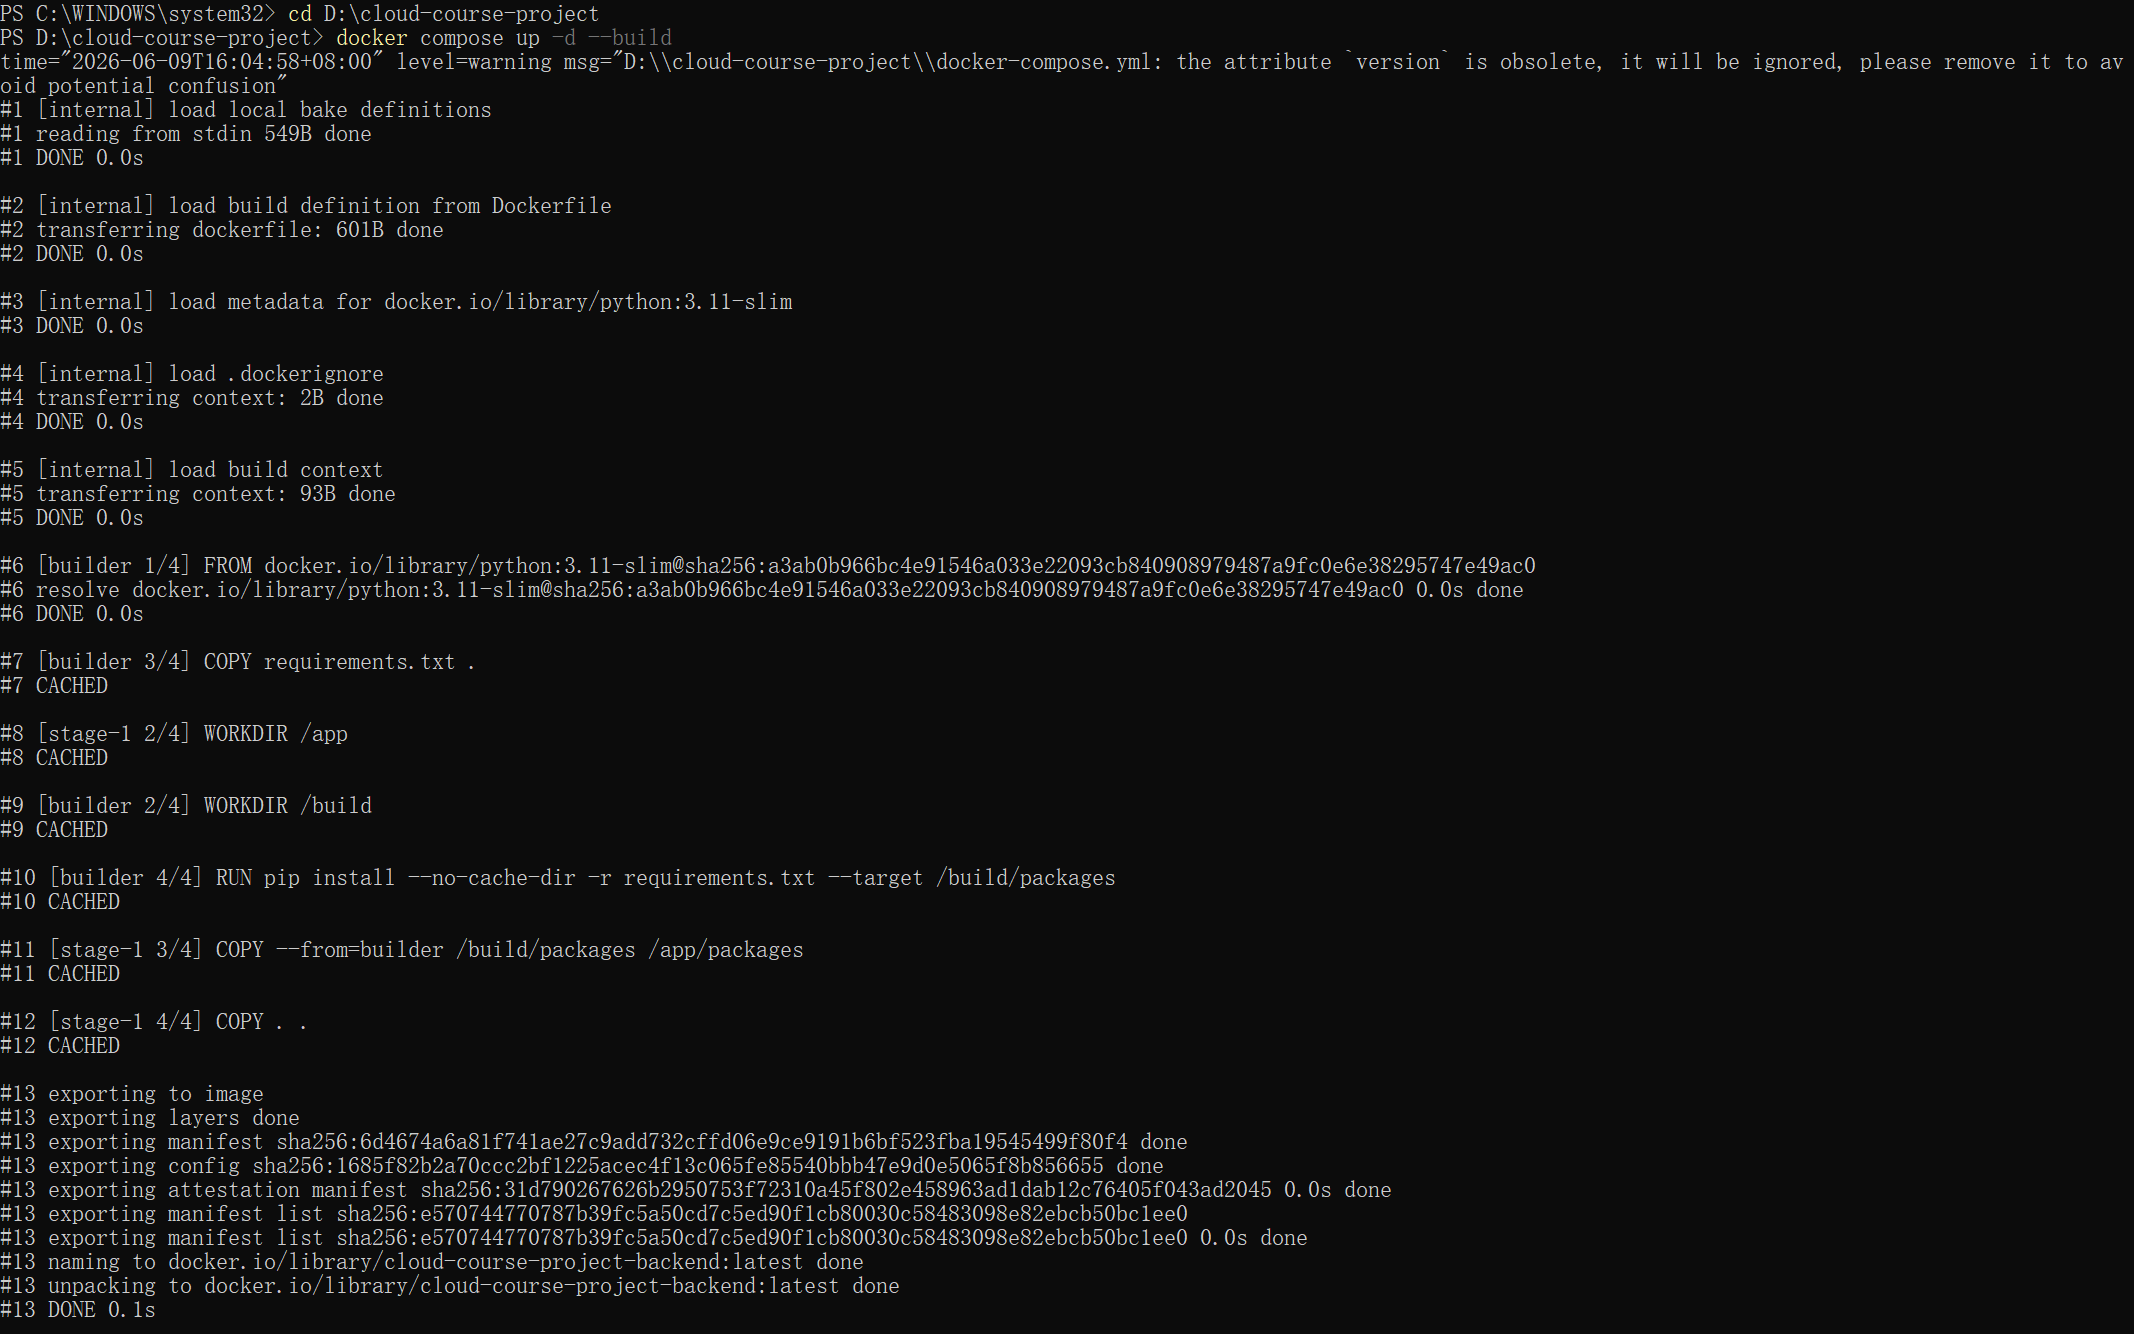
\includegraphics[width=0.92\textwidth]{assets/report_figures/overview-compose.png}
  \caption{Docker Compose 本地联调启动成功截图}
  \label{fig:overview-compose}
\end{figure}

\begin{figure}[H]
  \centering
  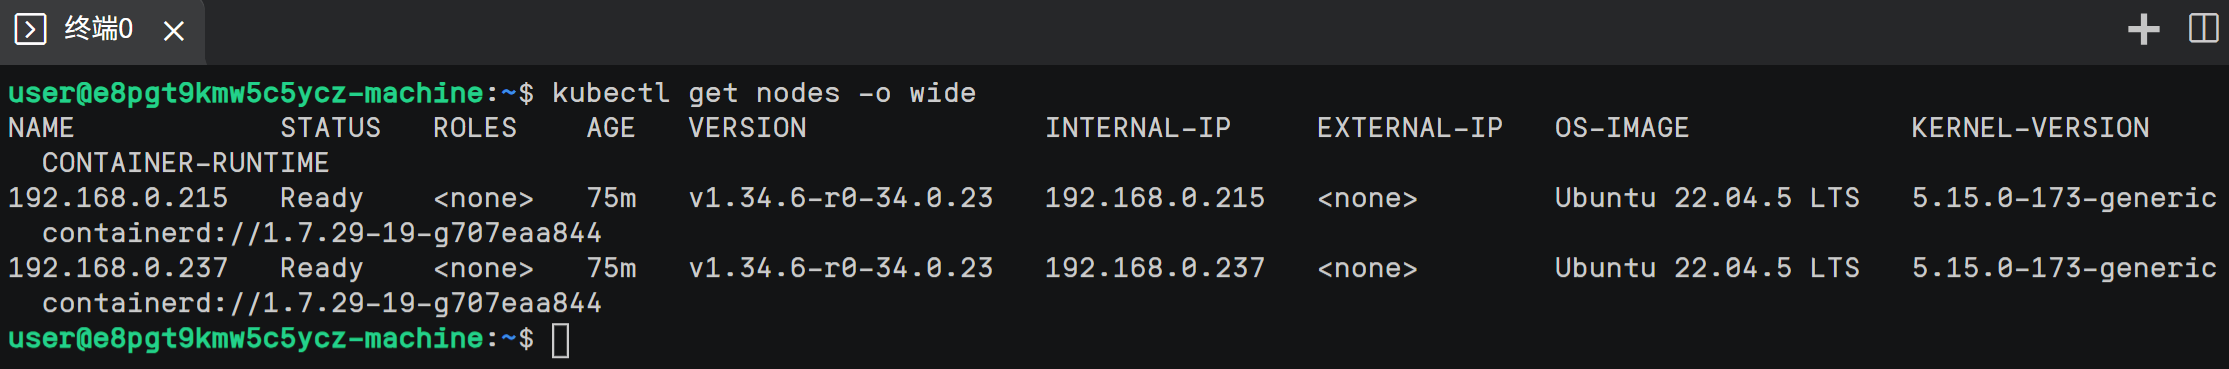
\includegraphics[width=0.92\textwidth]{assets/report_figures/overview-nodes-ready.png}
  \caption{CCE 集群两个 Worker 节点 Ready 验证截图}
  \label{fig:overview-nodes-ready}
\end{figure}

\begin{figure}[H]
  \centering
  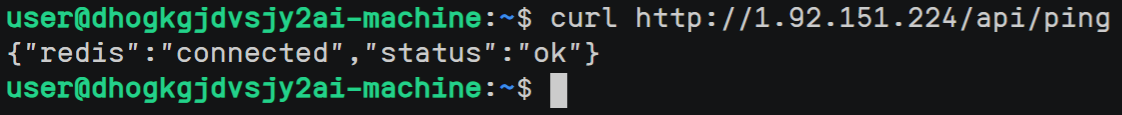
\includegraphics[width=0.92\textwidth]{assets/report_figures/overview-api-ping.png}
  \caption{通过 ELB 公网入口访问后端接口的验证截图}
  \label{fig:overview-api-ping}
\end{figure}

\subsubsection{代码仓库与报告材料说明}

本项目的代码与实验材料统一保存在课程设计仓库中。仓库根目录包含 `backend`、`frontend`、`k8s`、`spark`、`figures`、`figures\_A` 等目录，分别用于保存后端应用、前端静态页面、Kubernetes 资源文件、Spark 分析脚本和实验截图。后端部分以 Flask 提供 `/api/ping` 接口，并通过 Redis 验证服务间通信；前端部分基于 Nginx 提供静态页面和反向代理配置；`k8s` 目录保存 Deployment、Service、ConfigMap、Secret、PVC、HPA 等 YAML 文件；`spark` 目录保存 WordCount 示例、SparkApplication 模板和豆瓣电影数据分析脚本。

报告截图主要来自 `figures` 和 `figures\_A` 目录。`figures/T1` 保存应用容器化、本地联调和 SWR 镜像推送相关截图；`figures\_A/T2` 至 `figures\_A/T5` 保存 CCE 集群、应用部署、Redis 持久化和 ConfigMap Volume 挂载相关截图。后续章节将根据任务书验收要求插入截图，并在正文中说明截图反映的关键信息，例如 Pod 状态、Service 类型、ELB 公网 IP、PVC Bound 状态、Redis 数据持久化结果以及接口返回值等。通过这种组织方式，报告正文、代码文件和截图证据之间形成一一对应关系，便于检查和答辩说明。
